%==============================================================================
% presentation.tex
%==============================================================================


%==============================================================================
% Configuration
%==============================================================================

% Internationalisation
\usepackage[utf8]{inputenc}
\usepackage[T1]{fontenc}
% \usepackage[ngerman]{babel}

% Different packages
\usepackage{url}
\usepackage{color,listings,paralist}
\usepackage{enumerate}
\usepackage{tabularx}
\usepackage{alltt}

% Use default Acrobat reader fonts
\usepackage{mathpazo}

% Use CM fonts (increases document size)
\usepackage{ae}

% Use images
\usepackage{graphicx}

% Configure beamer
\usetheme[secheader]{Ikhono}
\usefonttheme[onlylarge]{structurebold}
\setbeamertemplate{navigation symbols}{}

% Variables
\providecommand{\Title}{Parallel Programming}
\providecommand{\Subtitle}{Recitation Session 7}
\providecommand{\Author}{Thomas Weibel <weibelt@ethz.ch>}
\providecommand{\Institute}{Laboratory for Software Technology, \\
  Swiss Federal Institute of Technology Z\"urich}
\providecommand{\Date}{April 22, 2010}

% PDF settings
\hypersetup{
  pdftitle={\Title, \Subtitle},
  pdfauthor={\Author},
  pdfsubject={\Institute},
  pdfkeywords={parallel programming} 
}

% Titlepage
\title{\Title}
\subtitle{\Subtitle}
\author{\Author}
\institute{\Institute}
\date{\Date}

% Listings
\lstdefinestyle{Default}{
  language=Java,
  tabsize=2,
  mathescape=true,
  inputencoding=utf8,
  showstringspaces=false,
  fontadjust=true,
  basicstyle=\ttfamily,
  keywordstyle=\color{blue}\bfseries,
}
\lstset{style=Default}


%==============================================================================
% Document
%==============================================================================

\begin{document}


% Titlepage
\begin{frame}[plain]
  \titlepage
\end{frame}


\section*{Introduction}

\begin{frame}{Executive Summary}
  \begin{itemize}
  \item TODO
  \end{itemize}
\end{frame}


\section{Determining when a Thread has finished}

\begin{frame}{Outline}
  \tableofcontents[current]
\end{frame}

\begin{frame}[fragile]{\lstinline{isAlive()}}
\begin{lstlisting}
// Create and start a thread 
Thread thread = new MyThread(); 
thread.start(); 

// Check if the thread has finished 
// in a non-blocking way 
if (thread.isAlive()) { 
  // Thread has not finished 
} else { 
  // Finished 
} 
\end{lstlisting}
\end{frame}

\begin{frame}[fragile]{\lstinline{join(delayMillis)}}
\begin{lstlisting}
// Wait for the thread to finish but don't 
// wait longer than a specified time 
long delayMillis = 5000; // 5 seconds 
try { 
  thread.join(delayMillis); 
  if (thread.isAlive()) { 
    // Timeout occurred, 
    // thread has not finished 
  } else { 
    // Finished 
  } 
} catch (InterruptedException e) { 
  // Thread was interrupted 
} 
\end{lstlisting}
\end{frame}

\begin{frame}[fragile]{\lstinline{join()}}
\begin{lstlisting}
// Wait indefinitely for the thread to finish 
try { 
  thread.join(); 
  // Finished 
} catch (InterruptedException e) { 
  // Thread was interrupted 
} 
\end{lstlisting}
\end{frame}


\section{Volatile}

\begin{frame}{Outline}
  \tableofcontents[current]
\end{frame}

\begin{frame}{The Volatile Returns}
  \begin{itemize}
  \item Volatile variables are not cached in registers or in
    caches where they are hidden from other processors
  \item A read of a volatile variable always returns the most recent
    write by any thread
  \end{itemize}

  \vspace{\stretch{1}}
  
  \begin{center}
    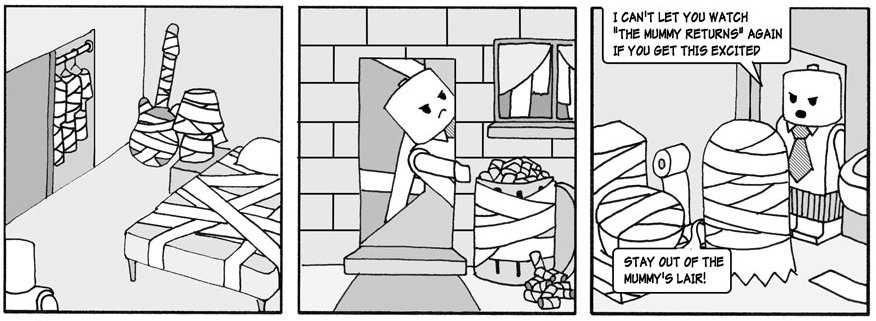
\includegraphics[width=\textwidth]{figures/the-mummy-returns} \\
    \tiny{Source: \url{http://thescope.ca/comics/everybodycheerup/the-mummy-returns}}
  \end{center}
\end{frame}

\begin{frame}[fragile]{Example}
\begin{lstlisting}[basicstyle=\fontsize{7}{9}\selectfont\ttfamily]
public class ShutdownDriver {
  boolean shutdown = false;

  public static void main(String[] args) throws InterruptedException {
    ShutdownDriver driver = new ShutdownDriver();
    new BusyTask(driver).start();
    Thread.sleep(2000);
    driver.shutdown = true;
  }
}

public class BusyTask extends Thread {
  private ShutdownDriver driver;

  public BusyTask(ShutdownDriver driver) {
    this.driver = driver;
  }

  public void run() {
    while (!driver.shutdown) {}
    System.out.println("Busy task stopped!");
  }
}
\end{lstlisting}
\end{frame}

\begin{frame}[fragile]{Example: Volatile}
\begin{lstlisting}[basicstyle=\fontsize{7}{9}\selectfont\ttfamily]
public class ShutdownDriver {
  volatile boolean shutdown = false;

  public static void main(String[] args) throws InterruptedException {
    ShutdownDriver driver = new ShutdownDriver();
    new BusyTask(driver).start();
    Thread.sleep(2000);
    driver.shutdown = true;
  }
}

public class BusyTask extends Thread {
  private ShutdownDriver driver;

  public BusyTask(ShutdownDriver driver) {
    this.driver = driver;
  }

  public void run() {
    while (!driver.shutdown) {}
    System.out.println("Busy task stopped!");
  }
}
\end{lstlisting}
\end{frame}

\begin{frame}{Synchronization}
  \begin{block}{Reading}
    Reading a volatile field is like acquiring a lock: The working
    memory is invalidated and the volatile field’s current value is
    reread from memory
  \end{block}

  \vspace{\stretch{1}}

  \begin{block}{Writing}
    Writing a volatile field is like releasing a lock: the volatile
    field is immediately written back to memory
  \end{block}
\end{frame}

\begin{frame}{Limitations}
  \begin{itemize}
  \item Although reading and writing a volatile field has the same
    effect on memory consistency as acquiring and releasing a lock,
    multiple reads and writes are not atomic
  \item For example, if \lstinline!x! is a volatile variable, the
    expression \lstinline!x++!  will not necessarily increment
    \lstinline!x! if concurrent threads can modify \lstinline!x!
  \item One common usage pattern for volatile variables occurs when a
    field is read by multiple threads, but only written by one
  \end{itemize}

  \vspace{\stretch{1}}

  \begin{alertblock}{No Atomicity!}
    \lstinline!volatile! alone is not strong enough to implement a
    counter, some form of mutual exclusion is needed as well
  \end{alertblock}
\end{frame}


\section{Last Assignment}

\begin{frame}{Outline}
  \tableofcontents[current]
\end{frame}

\begin{frame}{TODO}
  \begin{itemize}
  \item TODO
  \end{itemize}
\end{frame}


\section{TODO}

\begin{frame}{Outline}
  \tableofcontents[current]
\end{frame}

\begin{frame}{TODO}
  \begin{itemize}
  \item TODO
  \end{itemize}
\end{frame}


\section*{Outro}

\begin{frame}{Summary}
  \begin{itemize}
  \item TODO
  \end{itemize}
\end{frame}

\end{document}
